\chapter{Introduction}
\label{cha:100}
The goal of this project is to combine two different techniques (Grammatical Evolution and Proximal Policy Optimization) to optimize a policy, trying to exploit the best sides of both with the aim of making the process as fast and stable as possible. In particular the policies (expressed at high-level with decision trees) are built and optimized with Grammatical Evolution, an evolutionary algorithm which takes inspiration from the biological world. This algorithm performs mutations and crossovers on the individuals generation after generation, modifying the structure of the trees adding new genetic material or mixing that of two different individuals. During some specific generations, it's also applied Proximal Policy Optimization, which is a technique based on gradient ascent that modifies the values stored in the nodes of a decision tree, changing its behaviour in the environment and leaving its structure unchanged.

Doing this work of thesis, I tried to see if it is worth using these two algorithms combined together compared to using only Grammatical Evolution, making an analysis of the results in different environments to understand when this approach could work well and when not, and in the latter case, understand why it didn't work.

In this chapter there are all the definitions of algorithms, machine learning techniques and models used. The second chapter explains the parameters used in the main algorithm and how all the models and the interfaces have been changed to be able to link PPO algorithm to the principal evolutionary process. The third chapter covers the part concerning PPO, expounding the original algorithm and the modified version inspired by A. Silva et al. in \cite{silva} and the way I connected it with Grammatical Evolution, focusing on the difficulties encountered during this process. The fourth chapter deals with testing the algorithm in its entirety in different environments with varying complexity and showing the results obtained. In the last section of this chapter there is also the interpretability study for the best trees obtained with PPO. Finally, in the conclusion, there are some suggestion to improve the work that has been done.


\section{Reinforcement learning}
\label{sec:110}
The main context for this project falls into the category of Reinforcement learning (RL) tasks.

Reinforcement learning is learning what to do—how to map situations to actions—so as to maximize a numerical reward signal. The learner is not told which actions to take, but instead must discover which actions yield the most reward by trying them. In the most interesting and challenging cases, actions may affect not only the immediate reward but also the next situation and, through that, all subsequent rewards. These two characteristics—trial-and-error search and delayed reward—are the two most important distinguishing features of reinforcement learning \cite{sutton}.


\section{Markov Decision Process}
\label{sec:120}
The RL problem is abstracted as a Markov Decision Process (MDP), which is a five-tuple \(<\)\textit{S}; \textit{A}; \textit{P}; \(\gamma\); \textit{R}\(>\) defined as follows: \textit{S} is the set of states; \textit{A} is the set of actions; \textit{P} : \textit{S} \(\times\) \textit{A} \(\times\) \textit{S} \(\rightarrow\) [0, 1] is the transition matrix describing the probability that taking action \textit{a} \(\in\) \textit{A} in state \textit{s} \(\in\) \textit{S} results in state \textit{s'} \(\in\) \textit{S}; \(\gamma\)  \(\in\) [0, 1] is the discount factor defining the trade-off between immediate and future reward; and \textit{R} : \textit{S} \(\times\) \textit{A} \(\rightarrow\) \(\mathbb{R}\) is the function dictating the reward an agent receives by taking action \textit{a} \(\in\) \textit{A} in state \textit{s} \(\in\) \textit{S}. The goal is to learn a policy, \(\pi\) : \textit{S} \(\rightarrow\) \textit{A}, that prescribes which action to take in each state to maximize the agent’s long-term expected reward \cite{silva}.


\section{Grammatical Evolution}
\label{sec:130}
The principal algorithm used to evolve DTs is called Grammatical evolution (GE).

Grammatical evolution is an evolutionary algorithm that can evolve complete programs in an arbitrary language using a variable-length binary string. The binary genome determines which production rules in a Backus-Naur form grammar definition are used in a genotype-to-phenotype mapping process to a program \cite{neill}.

However, for the purpose of this project some modifications were done to the original algorithm; the key parts of the algorithm design are listed below:
\begin{itemize}
  \item The genotype has fixed length and is encoded as a list of codons, represented as integers
  \item Uniform mutation class is used as mutation operator; it mutates each gene depending on a probability passed in the configuration file
  \item  One-point crossover class is used as a crossover operator; this operator defines a random cutting point and creates two individuals by mixing the two sub-string of the genotype
  \item Replace operator works as follow: iterates through offspring and replaces the parents if the new individual is better, according to their fitness evaluation (i.e. the reward obtained in the environment)
\end{itemize}


\section{Proximal Policy Optimization}
\label{sec:140}
Proximal Policy Optimization (PPO) is a policy gradient method for reinforcement learning, which alternate between sampling data through interaction with the environment, and optimizing a “surrogate” objective function using stochastic gradient ascent \cite{schulman}.

The algorithm was modified to accept DTs (more precisely Differentiable Decision Trees (DDTs), which are explained in the section below), because normal DTs are not differentiable and the algorithm is based on gradient ascent and backpropagation. For more information about how I modified PPO, see the following chapter.


\section{Decision Tree}
\label{sec:150}
The model used as a controller to move the actor into the environment is a decision tree (DT), because of its ease of use and, in particular, its interpretability. So, what exactly is a DT?

A DT is an acyclic, directed graph that takes in input an example \textit{x}, performs a forward recursion starting from the root and returns a label \textit{y} (for this work, the example \textit{x} is the state \textit{s} \(\in\) \textit{S} and the label \textit{y} is the action \textit{a} \(\in\) \textit{A} in a MDP). There are two types of nodes: decision nodes with outdegree equals to 2 and leaves with outdegree equals to 0. All the nodes present in a DT have an indegree of one, except for the root, whose indegree is zero. Decision nodes are represented by Boolean expression where, in the case of orthogonal conditions like the ones used for this work, only one \textit{input\_feature} (\textit{x}) selected from the state space is compared with a real value named \textit{split\_value} (\(\phi\)). This type of comparison produces for the note an orthogonal hyperplane that splits the two input classes. Proceeding with the description, the left edge of every decision node is marked as \textit{TRUE}, ergo if the Boolean function is evaluated as \textit{True}, then the next node that it will be considered will be the left child of the current node, instead the right edge is marked as \textit{FALSE} with a similar definition. Finally, the leaves store a label which is , as I said before, the action that the agent has to execute in that particular state.

An example of a decision tree is shown in Figure \ref{fig:dt}

\begin{figure}[h!]
    \centering
    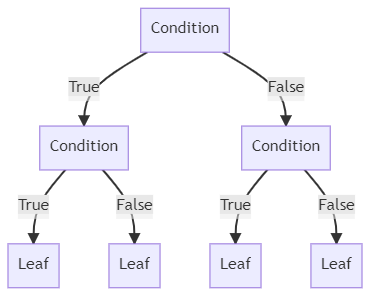
\includegraphics[width=0.5\linewidth]{images/DecisionTree.png}
    \caption{Example of decision tree model}
    \label{fig:dt}
\end{figure}

\newpage

\section{Differentiable Decision Tree}
\label{sec:160}
In order to apply a policy gradient method such as PPO, which cannot work with discrete DTs because of was designed for neural networks, DTs require some modification to get the so-called Differentiable Decision Trees (DDTs).

The approach proposed first in \cite{suarez} and thereafter taken and used by A. Silva et al. in \cite{silva} is to replace the Boolean condition in the decision nodes with a sigmoid activation function.

This method has also been used for this work.
\newpage
